\section{Conjecture sur l'erreur de généralisation}


\begin{lemme}[Généralisation du lemme de Hoeffding]
  \label{b:lem:hoeffding}
  Ce lemme généralise le lemme de Hoeffding à un espace vectoriel de dimension arbitraire
  $\Q$. Soit un vecteur aléatoire $Q\in\Q$ tel que $\nq{Q}\leq\beta$ et $\E Q = 0$. Alors pour tout
  $t\in\Q$, 
  \begin{equation}
    \E e^{\inp{t,Q}} \leq \exp\left(\frac{\beta^2\|t\|^2}{2}\right).
  \end{equation}
  En effet, on sait que par définition de la convexité de la fonction exponentielle, pour
  tout $s\in[0,1]$,
  \begin{equation}
    \exp(sa + (1-s)b) \leq s\exp a + (1-s)\exp b.
  \end{equation}
  Donc en définissant $g:\{q \in \Q:\|q\|\leq\beta\}\to[0,1]$ par
  \begin{equation}
    g(q) = \frac{1}{2}\left(\frac{\inp{t,q}}{\beta\|t\|} + 1\right)
  \end{equation}
  et en posant $a = \beta\|t\|$ et $b = -\beta\|t\|$, alors pour tout $q \in \Q$,
  \begin{gather}
    a g(q) = \frac{1}{2}(\inp{t,q} + \beta\|t\|),\\
    b (1-g(q)) = - \frac{1}{2}(\beta\|t\| - \inp{t,q}),
  \end{gather}
  et donc
  \begin{equation}
    \exp(ag(q) + (1-g(q))b) = e^{\inp{t,q}}.
  \end{equation}
  La branche droite de l'inégalité devient quant à elle
  \begin{equation}
    \left(\frac{\inp{t,q}}{\beta\|t\|} + 1\right)e^{\beta\|t\|} + \left(1-\frac{\inp{t,q}}{\beta\|t\|}\right)e^{-\beta\|t\|}
  \end{equation}
  et donc, puisque $\E\inp{t,Q} = \inp{t,\E Q} = 0$, 
  \begin{align}
    \E e^{\inp{t,Q}} &\leq \E\left(\left(\frac{\inp{t,Q}}{\beta\|t\|} + 1\right)e^{\beta\|t\|} +
                       \left(1-\frac{\inp{t,Q}}{\beta\|t\|}\right)e^{-\beta\|t\|}\right)\\
                     &= e^{\beta\|t\|} + e^{-\beta\|t\|}\\
                     &= e^{\phi(\beta\|t\|)}
  \end{align}
  où $\phi(x) = \log(e^{x} + e^{-x})$. Or, avec le résultat de \cite{mohri2012foundations},
  p.~370, on a $\phi(x) \leq x^2/2$, d'où on tire le résultat annoncé.
\end{lemme}

\begin{lemme}[Généralisation de la borne de Chernoff]
  \label{b:lem:chernoff}
  Ce lemme généralise la borne de Chernoff à un espace vectoriel de dimension arbitraire
  $\Q$. Soit un vecteur aléatoire $Q \in \Q$. Alors l'évènement $\|Q\| \geq \epsilon$ aura lieu si et
  seulement s'il existe $t \in \Q$, $\|t\|=1$ tel que $\inp{t,Q} \geq \epsilon$. Ainsi, pour tout
  $s>0$, en employant l'inégalité de Markov, 
  \begin{align}
    \pp\{\|Q\| \geq \epsilon\} &= \pp\{s\inp{t,Q} \geq s\epsilon\} = \pp\{e^{s\inp{t,X}} \geq e^{s\epsilon}\}\\
                     &\leq e^{-s\epsilon}\E e^{\inp{t,Q}}.
  \end{align}
\end{lemme}

\begin{lemme}[Généralisation de l'inégalité de McDiarmid]
  \label{b:lem:mcdiarmid}
  L'inégalité de McDiarmid peut également se généraliser à des fonctions prenant leurs
  valeurs dans des espaces vectoriels À élaborer!

  Soit une distribution $\mathscr{F}$ à valeur dans un espace quelconque $\bm F$, un
  espace vectoriel $\Q$ et une fonction $f:\bm F^n\to \Q$. S'il existe une constante
  $c\in\Re$ telle que pour deux ensembles d'échantillons \iid\ $\S_n \sim \mathscr{F}^n$ et
  $\S'_n$, où $\S_n$ et $\S'_n$ ne diffèrent que d'un seul point rééchantilloné de
  $\mathscr{F}$, on a
  \begin{equation}
    \|f(\S_n) - f(\S'_n)\| \leq c,
  \end{equation}
  alors pour tout échantillon aléatoire $\S_n\sim\mathscr{F}^n$, 
  \begin{equation}
    \pp\{\|f(\S_n) - \E f(\S_n)\| \geq \epsilon\} \leq \exp\left(-\frac{2\epsilon^2}{nc^2}\right).
  \end{equation}
\end{lemme}


\begin{lemme}[Borne sur la décision]
  \label{b:lem:qhnorm}
  Considérons le cas d'une utilité neutre au risque puisqu'on sait que toute solution à
  $\max_q\EU_\lambda(q)$ sera bornée par celle de $\max_q\EN_\lambda(q)$.  La stabilité de
  l'algorithme $\alg$ fournie par \cite{bousquet2002stability} établit que pour deux
  échantillons $\S_n$ et $\S_n'$ tirés de $M^n$ et ne différant que d'un seul point,
  \begin{equation}
    \|\alg(\S_n) - \alg(\S'_n)\| \leq \frac{\rmax\xi}{\lambda n}.
  \end{equation}
  En posant $\qh \sim \alg(M^n)$, on peut donc appliquer directement le résultat de
  l'inégalité de McDiarmid (\lemref{b:lem:mcdiarmid}) pour obtenir avec probabilité
  $1-\delta$ que
  \begin{equation}
    \|\qh - \E\alg(\S_n)\| \leq \frac{\rmax\xi}{\lambda}\sqrt{\frac{\log(1/\delta)}{2n}}.
  \end{equation}
  Or, $\alg$ est un estimateur non-biaisé de $\qsl$. En effet, pour une utilité neutre au
  risque,
  \begin{align}
    \E\alg(\S_n) &= \E_{M^n}\left(\frac{1}{2n\lambda}\sumi r_i\,\kappa(\cdot,x_i)\right)\\
                 & =\frac{1}{n}\sumi \frac{1}{2\lambda}\E_M(R\,\kappa(\cdot,X))\\
                 & =\frac{1}{n}\sumi \qsl\\
                 &=\qsl.
  \end{align}
  On obtient ainsi
  \begin{equation}
    \|\qh - \qsl\| \leq \frac{\rmax\xi}{\lambda}\sqrt{\frac{\log(1/\delta)}{2n}}.
  \end{equation}
\end{lemme}

% \begin{numex}{Convergence de $\qh$ vers $\qsl$}
%   La propriété du \lemref{b:lem:qhnorm} s'illustre particulièrement bien dans le cas où
%   $M$ n'est formé à ses marges que de distributions Rademacher. Ainsi, dans la
%   \figref{fig:normqhqsl}, une distribution de marché à deux variables d'information
%   indépendantes et toutes deux de corrélation $\rho=0.5$ avec $R$ sous copule gaussienne a
%   été simulée \num{10000} fois, pour constituer une ``vraie'' distribution pour laquelle
%   $\qsl$ peut être calculé; \num{2000} échantillons de $\S_n$ ont été simulés.
% \begin{figure}
%   \centering
%   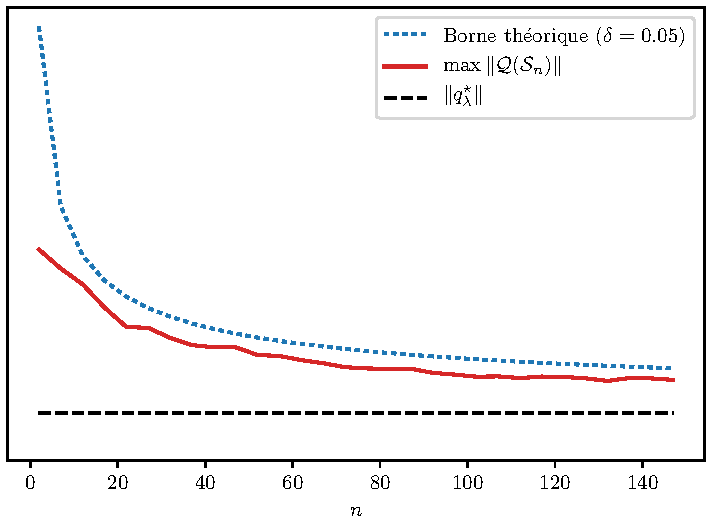
\includegraphics[width=0.7\textwidth]{../../experiments/fig/normqhqsl.pdf}
%   \caption{Illustration du \lemref{b:lem:qhnorm}.}
%   \label{fig:normqhqsl}
% \end{figure}
% \end{numex}


\begin{lemme}
  La solution $\qh_1$ de
  \begin{equation}
    \maximizeEquation[q \in \Q]{\EN_\lambda(q) = \hE\braket{q|t} - \tfrac{\lambda}{2}\|q\|^2.}
  \end{equation}
  est donnée par
  \begin{equation}
    \bra{\qh_1} = \lambda^{-1}\hE\bra{t}
  \end{equation}
  où $\bra{x_i} = \kappa(x_i,\cdot)$ est l'élément dual de $x$ sous $\Q$. Sous un noyau linéaire cela
  revient donc à 
  \begin{equation}
    \qh_1^T = \lambda^{-1}\hat\E(r^Tx)
  \end{equation}
  c'est à dire la covariance décentrée entre $r$ et $x$. On observera aussi que
  \begin{equation}
    \EN = \lambda\braket{\qh_1|\cdot}.
  \end{equation}
  et donc que
  \begin{equation}
    \EN(\qh_1) = \lambda\|\qh_1\|^2.
  \end{equation}
\end{lemme}

\begin{proof}
  Si on considère un déplacement de décision $\qh_1 + \Delta q$, alors par linéarité le premier
  terme de l'objectif devient $\EN(\qh_1+\Delta q) = \EN(\qh_1) + \EN(\Delta q)$ et le terme de
  régularisation devient 
  \begin{equation}
    -\lambda/2\|\qh_1 + \Delta q\|^2 = -\lambda/2\|\qh_1\|^2 - \lambda\braket{\qh_1|\Delta q} - \lambda/2\|\Delta q\|^2.
  \end{equation}
  On a donc
  \begin{align}
    \EN_\lambda(\qh_1)  - \EN_\lambda(\qh_1+\Delta q) &= -\EN(\Delta q) + \lambda\braket{\qh_1|\Delta q} + \lambda/2\|\Delta q\|^2\\
                                     &= -\lambda\braket{\qh_1|\Delta q} + \lambda\braket{\qh_1|\Delta q} +
                                       \lambda/2\|\Delta q\|^2\\
                                     &= \lambda/2\|\Delta q\|^2 \geq 0,
  \end{align}
  Ce qui entraîne $\EN_\lambda(\qh_1) \geq \EN_\lambda(\qh_1 + \Delta q)$.
\end{proof}

\begin{lemme}[Borne sur la décision utilitaire]
  \label{lem:rn}
  Pour toute fonction d'utilité $u$ respectant les hypothèses,
  \begin{equation}
    \|\qh_1\| \geq \|\qh_u\|.
  \end{equation}
  Ce lemme entraîne notamment que l'utilité en échantillon $\hEU(\qh_u) \leq \hEN(\qh_1)$:
  puisque $u(x) \leq x$,
  \begin{align}
    \hEU(\qh_u)&\leq \hEN(\qh_u) = \lambda\braket{\qh_1,\qh_u} \leq \lambda\|\qh_1\|\|\qh_u\| \leq \lambda\|\qh_1\|^2\\
               &=  \hEN(\qh_1)
  \end{align}
\end{lemme}

\begin{proof}
  On note tout d'abord avec l'inégalité de Jensen que
  $u(\hEN(\qu)) \geq \hEU(\qu) \geq \lambda/2\|\qu\|^2 \geq 0$ puisque la valeur de l'objectif
  $\hEN_\lambda(q)$ est d'au moins 0 à $q=0$. Mais puisque $u$ a un sur-gradient de 1 à
  $0$, on déduit que $u(x) \geq 0$ entraîne $x \geq u(x)$. On a ainsi
  $\hEN(\qu) - \lambda/2\nq{\qu}^2 \geq 0$. Ce qui entraîne alors que
  \begin{equation}
    \lambda\braket{\qh_1|\qh_u} \geq \lambda/2\|\qh_u\|^2
  \end{equation}
  Mais par Cauchy-Schwartz, on a aussi
  \begin{equation}
    \|\qh_1\|\|\qh_u\| \geq \braket{\qh_1,\qh_u} \geq \|\qh_u\|^2/2
  \end{equation}
  Et donc
  \begin{equation}
    \|\qh_1\| \geq \|\qh_u\|/2.\qedhere
  \end{equation}
\end{proof}


\begin{lemme}
L'erreur de généralisation du problème averse au risque est bornée par celle du problème
neutre au risque:
\begin{equation}
  \hEU(\qu) - \EU(\qu) \leq \gamma(\hEN(\qn) - \EN(\qn)).
\end{equation}
\end{lemme}
\begin{proof}
  Puisque $u$ est monotone, on peut tout d'abord noter que pour tout $r+\Delta \in \R$, on a
  l'inégalité $u(r+\Delta) \leq u(r) + \Delta \partial u(r)$. Ainsi, pour deux variables aléatoires $R_1,R_2 \in
  \R$, en posant $\Delta = R_1-R_2$, on a nécessairement
  \begin{equation}
    u(R_1) - u(R_2) \leq \partial u(R_2) (R_1 -R_2) \leq \gamma(R_1 - R_2),
  \end{equation}
  par définition du coefficient Lipschitz. On tire donc
  \begin{equation}
    \E u(R_1) - \E u(R_2) \leq \gamma(\E R_1 - \E R_2). 
  \end{equation}
  En appliquant cette inégalité aux opérateurs $\hEU$ et $\EU$ on obtient alors
  \begin{align}
    \hEU(\qu) - \EU(\qu) &\leq \gamma(\hEN(\qu) - \EN(\qu))\\
                         &= \gamma\lambda(\braket{\qh_1|\qu} - \braket{\qsl|\qu}).
  \end{align}
  Mais par le \lemref{lem:rn}, $\braket{\qh_1|\qu} \geq 0$ et $\|\qu\| \leq 2\|\qh_1\|$. 
\end{proof}



%%% Local Variables:
%%% mode: latex
%%% TeX-master: "memoire"
%%% End:
